\setchapterpreamble[u]{%
\dictum[Johann Wolfgang von Goethe]{Es ist nicht genug, zu wissen, man muß auch anwenden; es ist nicht genug, zu wollen, man muß auch tun. \dots}}
\chapter{Implementierung} \index{Implementierung}\label{kap:implementierung}

\section{Configuration Management und Setup}\index{Configuration Managment}

\subsection{Versionsverwaltung}\index{Versionsverwaltung}
\begin{quotation}
\enquote{A version control system (VCS) is a methodology or tool that helps you keep track of changes you make to the files in your project. In its simplest, manual form, a VCS is you creating a copy of the file you’re working with and adding the date and time to the end of it. \citep[S. 15][]{pragGit}}
\end{quotation}

Ein Versionskontrollsystem sollte in der Regel immer in der Softwareentwicklung eingesetzt werden um einerseits Änderungen nachvollziehen zu können, allerdings auch und vorallem um Änderungen rückgängig machen zu können die ggfs. fälschlicherweise durchgeführt wurden. Ferner ist es möglich verschiedene Versionen der Software gleichsam des Quellcodes zu führen und zu verwalten. Außerdem ermöglichen aktuelle \glslink{VCS}{Versionskontrollsysteme} die Zusammenarbeit mehrerer Entwickler am Quellcode. Hierbei hilft die Wiederherstellbarkeit und Nachvollziehbarkeit der Änderungen. 

\subsection{Versionsverwaltung mit GIT}\index{GIT}\index{Versionsverwaltung!verteilte Versionsverwaltung}

Was ist GIT?

GIT ist ein \gls{VCS}, kurz VCS, GIT ist darüberhinaus ein verteiltes \gls{VCS}, kurz DCVS.

\begin{quotation}
\enquote{Distributed version control systems (DVCSs) are no different in that respect. Their main goal is still to help us track changes we make to the projects we’re working on. The difference between VCSs and DVCSs is how developers communicate their changes to each other. \citep[S. 15][]{pragGit}}
\end{quotation}

In diesem Projekt ist kein verteiltes \gls{VCS} nötig, da es nur einen Bearbeiter der Daten und Quelltexte gibt. Es wurde dennoch gewählt, da es zum einen genau wie ein \enquote{normales}, folglich nicht verteiltes \gls{VCS} eingesetzt werden kann, der Autor mit diesem System sehr vertraut ist und ggfs. zukünftig auf diese Arbeit aufbauende oder weiterführende Projekte mit diesem System einfach weiterarbeiten können. 

Die Quelltexte dieser Arbeit sind bei einem frei verfügbaren \glslink{VCS}{Versionskontrollsystemanbieter} untergebracht. Das Repository kann mit dem Befehl aus \autoref{lst:klonendersourcen} geklont werden. Klonen bedeutet bei verteilten \glslink{VCS}{Versionskontrollsystem}, das gesamt Repository zu kopieren. Es kann dann auf diesem Repository lokal gearbeitet werden. 

Für mehr Informationen über GIT und den Funktionsumfang, sei auf entsprechende Literatur verwiesen \citep[vgl.][]{pragGit}.

 \begin{lstlisting}[caption=Klonen der Sourcen, language=XML, label=lst:klonendersourcen]
git clone https://username@bitbucket.org/ssobek/masterarbeit.git
 \end{lstlisting}   

\subsection{Build Management mit Maven}\index{Maven}

Was ist Maven?

\begin{quotation}
\enquote{Maven ist ein deklaratives Build Management System. Das heißt, es wird lediglich der Inhalt des Projekts beschrieben, nicht die Struktur oder die Abläufe, die zur Kompilierung und Veröffentlichung notwendig sind. Die Philosophie hinter Maven heißt \enquote{Konvention über Konfiguration} - Strukturen müssen nicht definiert werden, sondern sind vorgegeben. So wie die Projekt- und Verzeichnisstruktur ist auch die Reihenfolge der Arbeitsschritte vorgegeben, die Maven ausführt, um ein Projekt zu bauen. \citep[S. 27][]{Mitp-Verlag}}	
\end{quotation}

Wozu ist Maven in diesem Projekt nötig?

Maven ermöglicht konkret in diesem Projekt dem Betreuer, Professor oder Studenten, deren Arbeiten ggfs. aufbauend auf diese Arbeit sind, das Projekt standardisiert, einfach und ohne Kenntnisse von Maven oder anderen Werkzeugen zu erstellen. Maven findet dazu alle benötigten Abhängigkeiten automatisiert gemäß Konfiguration und erzeugt das Projekt. Es werden gemäß des standardisierten Buildablaufes von Maven mehrere Phasen durchlaufen, die beispielsweise sicherstellen, dass erst alle automatischen Tests erfolgreich durchlaufen sein müssen, bevor das Endprodukt erzeugt wird. 

In diesem Projekt wird Apache Maven in der Version 3 eingesetzt. 

Für mehr Informationen sei auf entsprechende Literatur verwiesen \citep[vgl.][]{Mitp-Verlag}.

\subsection{Apache Tomcat}\index{Apache Tomcat}
Als Web Container wird der \gls{Apache Tomcat} in der Version 7 eingesetzt. Die Installation wird in 
\autoref{kap:anhangtomcat} beschrieben. 
 
\subsection{Tests}\index{Tests}\index{Entwicklertest}

Einer der wichtigsten Punkte in der Softwareentwicklung ist das Testen. Es werden auschließlich Entwicklertests betrachtet. Hier gibt es zwei Bereiche, automatische Entwicklertests und manuelle Entwicklertests. 

\subsubsection{Automatische Entwicklertests mit JUnit}\index{Unit Test}\index{Integrationstest}

Für die automatischen Entwicklertests wird ein Framework namens JUnit eingesetzt. Der Vorteil ist, dass dieses Framework weit verbreitet, bekannt und ausgereift ist. 
Es gibt zwei Arten von Tests. Die \glspl{Unit-Test} und die \glspl{Integrationstest}. 

\glspl{Unit-Test} testen eine Komponente isoliert von allen abhängigen Komponenten. Das bedeutet, dass nur diese Komponente auf die korrekte Funktionsweise hin getestet wird. Jegliche Abhängigkeiten werden durch Mock- oder Fakeobjekte ersetzt, so dass ein genaue Testumgebung für diese Komponente simuliert werden kann. 

\glspl{Integrationstest} testen mehrere Komponenten im Verbund und testen Anwendungszenarien. Ein Beispiel ist ein Test, welcher auf der grafischen Benutzeroberfläche einsetzt, dort einen Knopf drückt (z.B. Benutzer anlegen) und durch alle Schichten hindurch bis hin zur Datenbank einen Eintrag in der Datenbank anlegt. Anschließend wird entweder in der Datenbank oder erneut auf der Benutzeroberfläche geprüft (Liste aller Benutzer), ob der Eintrag erzeugt wurde. 
Dies ist ein Beispiel wo die Gesamtapplikation integriert und somit lauffähig sein muss, damit man dieses Szenario testen kann. 
Ein Integrationstest ist es allerdings bereits schon dann, wenn automatisiert ein Datenzugriffsobjekt im Verbund mit der Datenbank getestet wird, da hier bereits mehrere Komponenten zusammen getestet werden. 

Mehr Informationen und einige Code-Beispiele in \autoref{anh:automatischeentwicklertests}.

\subsubsection{Manuelle Entwicklertests}\index{Manuelle Entwicklertests}

Bei manuellen Entwicklertests werden Testcases aus den Anforderungen abgeleitet. Diese Tests sind sogenannte Black Box Tests. Das bedeutet, dass das Objekt, welches getestet wird als Black Box betrachtet wird. Es sind keine technischen Details über Aufbau dieses Testobjektes bekannt und es werden keine Annahmen getroffen. Lediglich die Schnittstelle nach Außen wird betrachtet und gemäß Spezifikation der Ein- und Ausgangsdaten getestet. 

Die Testfälle und Ergebnisse finden sich in \autoref{anh:testszenarios}.

\subsubsection{Testtools}

Zum manuellem Testen werden verschiedene Tools verwendet. Diese müssen in der Lage sein, einen POST-Request an eine URL zu senden und ein XML, das Query-XML, als Payload mitzusenden.

\paragraph{CURL}\index{CURL}

Auf Linux-basierten Systemen kann das Werkzeug \enquote{curl} verwendet werden. Dieses Werkzeug liegt allen Linux oder Unix basierten Betriebssystemen in der Regel bei, oder kann einfach nachinstalliert werden. 

Je nach Betriebssystem wird das mittels Befehlszeile über einen sogenannten Paketmanager durchgeführt:
\begin{description}
\item[Ubuntu, Debian] apt-get install curl
\item[Fedora, RedHat, CentOs] yum install curl
\end{description}

Ein Beispielaufruf ist in \autoref{lst:curltest} zu sehen. Hier wird eine XML-Datei namens query\_class\_irdi.xml an die URL http://localhost:8080/rest/ws/query/ gesendet. 

\begin{lstlisting}[caption=CURL Test des REST Webservices, language=sh, label=lst:curltest]
curl -v -H "Content-Type: application/xml" -X POST --data "@src/test/resources/de/feu/plib/xml/query_class_irdi.xml" http://localhost:8080/rest/ws/query
 \end{lstlisting}   

\paragraph{Advanced REST Client} \index{Advanced REST Client}

Eine andere Möglichkeit den \gls{REST} Webservice zu testen ist ein Plugin des Browsers Chrome, genannt \enquote{Advanced REST Client}. Dieser kann auch einen POST-Request erzeugen und an eine URL senden. Die \autoref{fig:advancedrestclienttest} zeigt einen Test eines einfachen XML-Files. Dazu muss der XML Inhalt in das untere Eingabefeld unter dem Reiter \enquote{Payload} eingeben werden. Ferner muss der Content-Type auf \enquote{application/xml} gesetzt werden, um entsprechende HTTP-Header mitzuschicken, welche dem Webservice mitteilen, dass auch tatsächlich XML Daten kommen. 

\begin{figure}[htbp]
	\centering
		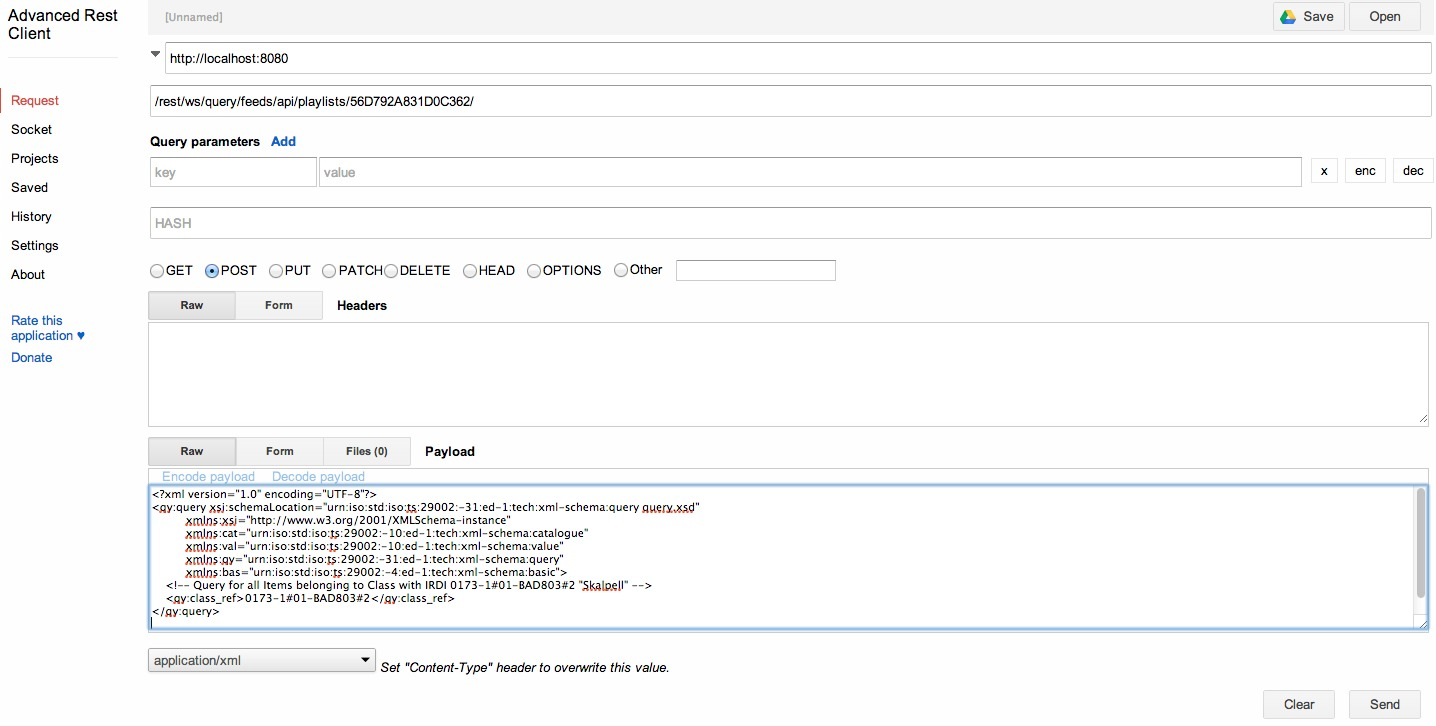
\includegraphics[width=0.98\textwidth]{images/advanced_rest_client_test.jpg}
	\caption{Advanced REST Client Test des Webservices}
	\label{fig:advancedrestclienttest}
\end{figure}

\section{Webservice}\index{Webservice}\index{REST!RESTful Webservice}\label{kap:webservice}

Wie in \autoref{sec:webservice} erwähnt, wurde entschieden einen \gls{REST}ful \gls{Webservice} zu erstellen. Dafür wurde das \gls{Jersey}-Framework ausgewählt. 

\begin{description}
\item[Zur Erklärung] Java unterstützt REST durch die Java Specification Request 311 (JSR)\footnote{Spezifikation ist zu finden unter: http://jcp.org/aboutJava/communityprocess/mrel/jsr311/index.html}. Diese Spezifikation wird JAX-RS - die Java API for RESTful Webservices genannt. Jersey ist die Referenzimplementierung, bereits in Java 6 integriert. Das auch der Grund, weshalb die Jersey Implementierung als Basis gewählt wurde.  
\end{description}

Folgende Schritte sind notwendig um einen \gls{REST}ful Webservice mit Jersey zu erstellen: 

\subsection{Servlet Konfiguration in web.xml} \index{Jersey}

In die Konfigurationsdatei web.xml des Webcontainers (hier \gls{Apache Tomcat}) muss das Servlet für \gls{Jersey} hinzugefügt werden, so dass \gls{Webservice} Anfragen an dieses Servlet möglich sind. 

\autoref{lst:jerseywebxmlconfig} zeigt den Ausschnitt aus der web.xml des \gls{PLIB}-Projektes. 

 \begin{lstlisting}[caption=Jersey Servlet Konfiguration in web.xml, language=XML, label=lst:jerseywebxmlconfig]
 <!-- configure jersey REST-Web Service Servlet -->
    <servlet>
        <servlet-name>jersey-servlet</servlet-name>
        <servlet-class>com.sun.jersey.spi.container.servlet.ServletContainer</servlet-class>
        <init-param>
            <param-name>com.sun.jersey.config.property.packages</param-name>
            <param-value>de.feu.plib.webservice.rest</param-value>
        </init-param>
        <load-on-startup>1</load-on-startup>
    </servlet>
 \end{lstlisting}   
 
Ferner muss in der web.xml ein sogenannter \enquote{Mappingeintrag} angelegt werden. Hierdurch wird dem Webserver mitgeteilt, welche \gls{URL}-Aufrufe an welches \gls{Servlet} zur Verarbeitung geleitet werden sollen. 
 
  \begin{lstlisting}[caption=Jersey Servlet Mappingkonfiguration in web.xml, language=XML, label=lst:jerseywebxmlconfigmapping]
    <servlet-mapping>
        <servlet-name>jersey-servlet</servlet-name>
        <url-pattern>/rest/*</url-pattern>
    </servlet-mapping>
 \end{lstlisting}  
 
Das Konfigurationbeispiel in \autoref{lst:jerseywebxmlconfigmapping}  besagt, dass das \gls{Servlet} mit dem Namen \enquote{jersey-servlet}, welches im Beispiel \autoref{lst:jerseywebxmlconfig}  konfiguriert wurde, alle Anfragen mit der URL \enquote{/rest/*} entgegennehmen soll. Das Muster \enquote{/rest/*} bedeutet, das beliebige URLs nach /rest/ akzeptiert werden. Zum Beispiel: \enquote{/rest/webservice} oder \enquote{/rest/service/name}.

Unter der Annahme, dass die Applikation auf dem lokalen Rechner installiert wurde und auf Port 8080 lauscht, der \gls{Applikationskontext} \enquote{plib-characteristic-query} ist, ergibt sich als aktuelle Gesamt-URL für den \gls{Webservice} der Applikation \enquote{http://localhost:8080/plib-characteristic-query/rest/}.
\index{Apache Tomcat!Applikationskontext} \todotext{Applikationskontext footnote}

\subsection{Webservice Klasse}
Der Einstiegspunkt für den \gls{Webservice} ist eine Klasse. Eine Applikation kann mehrere solcher Einstiegspunkte haben. Damit die Navigation von der \gls{URL} der Anfrage zur entsprechenden Klasse funktioniert, wird jede Klasse mittels Annotation markiert und ein weiterer Pfad-Präfix definiert. Das Beispiel 
\autoref{lst:jerseywebservice} zeigt, dass mittels @Path der Suffix /ws definiert wird. Das bedeutet, dass die Klasse QueryService den \gls{URI}-Pfad /ws zugewiesen bekommt. 
  \begin{lstlisting}[caption=Jersey Webservice Klasse, language=Java, label=lst:jerseywebservice]
...
@Path("/ws")
public class QueryService {
...
 \end{lstlisting}  
 
Somit ergibt sich als aktuelle Gesamt-\gls{URL} für den \gls{Webservice} der Applikation \\  \enquote{http://localhost:8080/plib-characteristic-query/rest/ws}.
 
Der nächste Schritt ist es, die entsprechenden Methode zu definieren, welche die Anfrage final entgegennimmt und verarbeitet (siehe \autoref{lst:jerseymethode}). 
 
  \begin{lstlisting}[caption=Jersey Methode, language=Java, label=lst:jerseymethode]
    @POST
    @Path("/query")
    @Consumes("application/xml")
    @Produces(MediaType.APPLICATION_XML)
    public String query(String queryXML) {
        LOGGER.info("Incoming query XML content :" + queryXML);
        QueryType queryType = unmarshall(queryXML);
        LOGGER.info("QueryType: " + queryType);
        CatalogueType catalogue = queryPipe.filter(queryType);

        LOGGER.info("Filled Catalogue: " + catalogue);
        String marshalledCatalogue = marshall(catalogue);

        LOGGER.info("Marshalled catalogue: " + marshalledCatalogue);
        return marshalledCatalogue;
    }
 \end{lstlisting}  

Die Konfiguration der Methode wird über \Gls{Annotation} vorgenommen. Nachfolgend die Erklärung der \Glspl{Annotation} aus \autoref{lst:jerseymethode}.

\begin{description}
\item[@POST] Definiert die \gls{HTTP-Methode}. Hier \gls{POST}. Einige weitere Möglichkeiten des \gls{HTTP}-Protokolls sind GET, PUT und DELETE
\item[@Path('/query')] Definiert den URL-Pfad Suffix für diese Methode. Um diese Methode als Web Service via \gls{HTTP} aufzurufen lautet die finale URL \enquote{http://localhost:8080/plib-characteristic-query/rest/query}. 
\item[@Consumes('application/xml')] Definiert den \gls{MIME-Type}\footnote{Internet Media Type oder auch Content-Type.}, welcher von diesem Service (diese Methode) konsumiert werden kann. Wird ein anderer Typ als POST an diesen Service geliefert, weist der Service diese Anfrage ab. 
\item[@Produces(MediaType.APPLICATION\_XML)] Definiert den \gls{MIME-Type} des Inhaltes, der vom Service als Antwort zurückgeliefert wird.  
\end{description}
\index{HTTP-Methode!GET}\index{HTTP-Methode!POST}\index{HTTP-Methode!PUT}\index{HTTP-Methode!DELETE}
\index{MIME-Type}

\section{Query-Verarbeitung}

Der \gls{Webservice}, welcher in \autoref{kap:webservice} beschrieben ist, nimmt in der Applikation das Query-XML-File entgegen. 
Die Struktur des XML-Files ist durch die query.xsd vorgegben \citep[27]{iso29002-31}. 

Der nächste Schritt ist es, diese XML-Datei zu verarbeiten. Dazu muss die XML-Datei geparsed und die Informationen des Queries in ein entsprechendes Modell überführt werden. Diesen Prozess nennt man \gls{Unmarshalling}. 

Die folgenden Schritte müssen für das \gls{Unmarshalling} durchgeführt werden.

\begin{enumerate}
\item Ein Modell in Java erstellen
\item XML parsen und in das Modell überführen
\item Validierung des Modells gemäß der Regeln aus Schema-Datei
\end{enumerate}

%modell
\subsection{Modell-Generierung}\label{sec:modellgenerierung}

Ein entsprechend valides Model anhand der XSD manuell in Java aufzubauen wäre sehr mühsam und fehleranfällig. Java liefert mit der \gls{JAXB} Bibliothek die Möglichkeit die Modellklassen von Java aus den XSDs zu generieren.

\subsubsection{Benötigte XSD-Dateien}

Die XSD-Dateien der ISO 29002-31 wurden freundlicherweise von Dr. Gerry Radack von der \gls{ECCMA} zur Verfügung gestellt. 

Die query.xsd referenziert die weiteren folgenden Schema-Dateien:
\begin{itemize}
\item basic.xsd
\item identifier.xsd
\item catalogue.xsd
\item value.xsd
\end{itemize}

\subsubsection{Generierung mit JAXB}\index{Codegenerierung}\index{JAXB}

Die Generierung startet man als Java Kommando in der Konsole, siehe \autoref{lst:jaxbgeneratemodel}.

\begin{lstlisting}[caption=JAXB Modellgenerierung mittels Konsolenbefehl, language=sh, label=lst:jaxbgeneratemodel]
xjc query.xsd -d plib-characteristic-data/ 
\end{lstlisting}

\subsubsection{Problem Namensräume}
Bei der Generierung wurde die folgende Fehlermeldung angezeigt:

\enquote{[ERROR] The package name iso.std.iso.ts.\_29002.\_\_-31.ed\_1.tech.xml\_schema.query used for this schema is not a valid package name. line 18 of file query.xsd}
  
Der Grund für den Fehler ist, dass in der query.xsd die \glslink{Namespace}{Namensräume}\footnote{Im weiteren Verlauf wird der englische Begriff Namespaces für Namensräume benutzt.} wie in  \autoref{lst:queryschemanamespace} definiert sind. Da JAXB die \Glspl{Namespace} nutzt um die entsprechenden Paketstrukturen für die Modelle in Java zu erstellen, schafft es JAXB nicht, diese in entsprechende valide Form umzuwandeln. Man erkennt es daran, dass aus 

\enquote{urn:iso:std:iso:ts:29002:-31:ed-1:tech:xml-schema:query} 

in der Fehlermeldung 

\enquote{iso.std.iso.ts.\_29002.\_\_-31.ed\_1.tech.xml\_schema.query} 

wird\footnote{Java Paketnamen enthalten als Trenner zwischen den Ebenen einen Punkt. Valide wäre z.B. iso.std.iso.ts.query}.
Der Bindestrich vor der 31 ist nicht als erstes Zeichen eines Unterpaketnamens erlaubt. Wenngleich man hier erwarten würde, dass dies abgefangen und entsprechend der Umwandlungsregeln in valide Bezeichner konvertiert wird, so führt eine Benamung der Pakete nach den \Glspl{Namespace} zu unübersichtlichen und nicht aussagekräftigen Paketstrukturen. \index{Namespace}

\begin{lstlisting}[caption=query.xsd Namespace Definitionen, language=XML, label=lst:queryschemanamespace]
<xs:schema xmlns:xs="http://www.w3.org/2001/XMLSchema"
           xmlns:qy="urn:iso:std:iso:ts:29002:-31:ed-1:tech:xml-schema:query"
           xmlns:cat="urn:iso:std:iso:ts:29002:-10:ed-1:tech:xml-schema:catalogue"
           xmlns:val="urn:iso:std:iso:ts:29002:-10:ed-1:tech:xml-schema:value"
           xmlns:bas="urn:iso:std:iso:ts:29002:-4:ed-1:tech:xml-schema:basic"
           xmlns:id="urn:iso:std:iso:ts:29002:-5:ed-1:tech:xml-schema:identifier"
           targetNamespace="urn:iso:std:iso:ts:29002:-31:ed-1:tech:xml-schema:query" elementFormDefault="qualified">
    <xs:import namespace="urn:iso:std:iso:ts:29002:-4:ed-1:tech:xml-schema:basic" schemaLocation="basic.xsd"/>
    <xs:import namespace="urn:iso:std:iso:ts:29002:-5:ed-1:tech:xml-schema:identifier" schemaLocation="identifier.xsd"/>
    <xs:import namespace="urn:iso:std:iso:ts:29002:-10:ed-1:tech:xml-schema:catalogue" schemaLocation="catalogue.xsd"/>
    <xs:import namespace="urn:iso:std:iso:ts:29002:-10:ed-1:tech:xml-schema:value" schemaLocation="value.xsd"/>
    ...
</xs:schema>    
\end{lstlisting}

Für dieses Problem gibt es zwei Lösungsoptionen. Entweder die \gls{Namespace}-Definitionen aller \Glspl{Namespace} in den XSD-Dateien anpassen oder die XSD-Dateien in der Form belassen und einen programmatischen Weg finden um die \Glspl{Namespace} umzudefinieren. 

Das Anpassen aller XSD-Dateien hat zwei große Nachteile.
\begin{enumerate}
\item Es ist aufwändig und fehleranfällig alle Dateien anzupassen. Diese haben wie in \autoref{lst:queryschemanamespace} zu sehen, Abhängigkeiten untereinander\footnote{Die Abhängigkeiten erfolgen über die xs:import Anweisungen. Damit werden weitere Schema-Dateien eingebunden und die entsprechenden Elemente nutzbar gemacht.}.
\item Änderungen an der lokalen Schemadatei machen mögliche spätere Integrationen einer neuen XSD-Version des ISO-Komitees schwierig.
\end{enumerate}

Zu bevorzugen ist eine konfigurierbare Generierung. \gls{JAXB} ermöglicht mit einem sogenanntem Binding-File\footnote{Ein Binding-File ist eine XML-Datei, welche gemäß JAXB eine Konfiguration für die Genierung ermöglicht.}, die \Glspl{Namespace} abzuändern. \autoref{lst:bindingfile} zeigt die Konfiguration. Die Generierung kann mit dem Shell-Befehl 

\enquote{xjc -b binding.xjb -d gen-src query.xsd} 

gestartet werden. \index{Binding} \index{JAXB}

\begin{lstlisting}[caption=Binding File binding.xjc, language=XML, label=lst:bindingfile]
<?xml version="1.0" encoding="UTF-8"?>
<jaxb:bindings xmlns:jaxb="http://java.sun.com/xml/ns/jaxb"
               xmlns:xsd="http://www.w3.org/2001/XMLSchema"
               xmlns:xjc="http://java.sun.com/xml/ns/jaxb/xjc"
               jaxb:version="2.0">
  <jaxb:bindings schemaLocation="query.xsd" node="/xsd:schema">
    <jaxb:schemaBindings>
      <jaxb:package name="de.feu.plib.xml.query" />
    </jaxb:schemaBindings>
  </jaxb:bindings>
  <jaxb:bindings schemaLocation="basic.xsd" node="/xsd:schema">
    <jaxb:schemaBindings>
      <jaxb:package name="de.feu.plib.xml.basic" />
    </jaxb:schemaBindings>
  </jaxb:bindings>
  <jaxb:bindings schemaLocation="catalogue.xsd" node="/xsd:schema">
    <jaxb:schemaBindings>
      <jaxb:package name="de.feu.plib.xml.catalogue" />
    </jaxb:schemaBindings>
  </jaxb:bindings>
  <jaxb:bindings schemaLocation="identifier.xsd" node="/xsd:schema">
    <jaxb:schemaBindings>
      <jaxb:package name="de.feu.plib.xml.identifier" />
    </jaxb:schemaBindings>
  </jaxb:bindings>
  <jaxb:bindings schemaLocation="value.xsd" node="/xsd:schema">
    <jaxb:schemaBindings>
      <jaxb:package name="de.feu.plib.xml.value" />
    </jaxb:schemaBindings>
  </jaxb:bindings> 
  
      <jaxb:globalBindings>
         <!-- let the classes implement serialiseable -->
        <jaxb:serializable uid="1" />
          <!-- let the classes extend own abstract class for providing some extra functionality for each one -->
     </jaxb:globalBindings>  
</jaxb:bindings> 
\end{lstlisting}

Wie man erkennen kann, wird für jede Schema Datei ein eigener Paketname definiert. Das hat den Vorteil, dass die einzelnen Datentypen aus den jeweiligen XSD-Dateien passend in eigene Pakete generiert werden und nicht alle in ein Verzeichnis. Das ist deutlich übersichtlicher. 

Die Modell-Dateien werden folgendermaßen abgelegt:

\begin{description}
\item[query.xsd] de.feu.plib.xml.query
\item[basic.xsd] de.feu.plib.xml.basic
\item[catalogue.xsd] de.feu.plib.xml.catalogue
\item[identifier.xsd] de.feu.plib.xml.identifier
\item[value.xsd] de.feu.plib.xml.value
\end{description}

Zeile 6-10 aus \autoref{lst:bindingfile} zeigt auf, wie im Binding-File ein anderer Paketname für die Datei query.xsd definiert werden kann. 

\subsection{Einbinden in Buildprozess mit Maven}\index{Maven}\index{Buildprozess}
Da als Build-Werkzeug \gls{Maven} verwendet wird, kann der gesamte Generierungsprozess darüber abgebildet werden. 

\subsubsection{Separates Source-Verzeichnis}\index{VCS}\index{Versionierung}
Die Standardprojektform eines \gls{Maven}-Projektes hat einen sogenannten Source-Folder (src). Darin befindet sich ein main-Folder. Dort werden die Klassen der Applikation abgelegt. Ferner beinhaltet der src-Folder einen test-Folder. Darin werden Testklassen abgelegt. 
Damit die generierten Sourcen klar von den anderen Source-Dateien getrennt sind, soll ein separates Source-Verzeichnis angelegt werden. Der weiterer Vorteil ist, dass dieser Folder beispielsweise auch vom \gls{VCS} ausgenommen werden kann, da diese Klassen während des Build-Prozesses jeweils generiert werden und somit keiner Versionierung bedürfen. Das wäre aufwändiger zu realisieren, wenn die Dateien exakt im gleichen Source-Folder generiert würden wo alle anderen Source-Dateien liegen\footnote{Hinweis: Moderne \gls{VCS} wie das eingesetzte GIT ermöglicht es nach Mustern Dateien oder Ordner von der Versionierung auszunehmen. Allerdings müsste das hier auf Paketbasis erfolgen, sozusagen ab de.feu.plib.xml.*, das macht die Umgebung im Ganzen komplexer}. 

\gls{Maven} bietet mittels des Plugins \enquote{build-helper-maven-plugin} die Möglichkeit, dies zu erzeugen. 
Die generierten Sourcen der XSD-Dateien werden in ein separates Verzeichnis namens \enquote{generated} erzeugt (siehe \autoref{lst:buildhelperplugin}). 

\begin{lstlisting}[caption=Build Helper Maven Plugin, language=, label=lst:buildhelperplugin]
<plugin>
    <groupId>org.codehaus.mojo</groupId>
    <artifactId>build-helper-maven-plugin</artifactId>
    <executions>
        <execution>
            <id>add-source</id>
            <phase>generate-sources</phase>
            <goals>
                <goal>add-source</goal>
            </goals>
            <configuration>
                <sources>
                    <source>src/main/generated</source>
                </sources>
            </configuration>
        </execution>
    </executions>
</plugin>
\end{lstlisting}

\subsubsection{JAXB Maven Plugin}\index{Maven-Plugin}

Um JAXB mit \gls{Maven} zu nutzen, muss das \gls{Maven}-Plugin \enquote{maven-jaxb2-plugin} in die \gls{pom} eingetragen werden. \autoref{lst:jaxbplugin} zeigt den XML-Auschnitt aus der \gls{pom}. \index{Maven!pom.xml}

\begin{lstlisting}[caption=JAXB Maven Plugin, language=XML, label=lst:jaxbplugin]
            <plugin>
                <groupId>org.jvnet.jaxb2.maven2</groupId>
                <artifactId>maven-jaxb2-plugin</artifactId>
                <version>0.8.0</version>
                <configuration>
                    <schemaDirectory>src/main/resources/schema</schemaDirectory>
                    <generateDirectory>src/main/generated</generateDirectory>
                    <removeOldOutput>true</removeOldOutput>
<!-- we do not use bindingDirectory as if we put the binding.xjb in the schema directory it will be taken -->
<!--                     <bindingDirectory>src/main/resources/binding</bindingDirectory> -->

<!--  Setting the generated package in pom will override what you set in binding.xjb file, thus commented out -->
<!--                     <generatePackage>de.feu.plib.jaxb</generatePackage> -->
                    <strict>false</strict>
                    <extension>true</extension>
                    <plugins>
                        <plugin>
                            <groupId>org.jvnet.jaxb2_commons</groupId>
                            <artifactId>jaxb2-basics</artifactId>
                            <version>0.6.2</version>
                        </plugin>
                        <plugin>
                            <groupId>org.jvnet.jaxb2_commons</groupId>
                            <artifactId>jaxb2-basics-annotate</artifactId>
                            <version>0.6.2</version>
                        </plugin>
                    </plugins>
                    <args>
                        <arg>-Xannotate</arg>
                        <arg>-XtoString</arg>
                    </args>
                </configuration>
                <executions>
                    <execution>
                        <id>generate</id>
                        <goals>
                            <goal>generate</goal>
                        </goals>
                    </execution>
                </executions>
            </plugin>    
\end{lstlisting}

\section{Abfrage der PLIB Prozeduren}\index{PLIB Prozeduren}\index{Oracle Prozeduren}\label{sec:abfrage_plib_prozeduren}

Die Anforderung ist es, so weit wie möglich die vorhandenen Prozeduren der PLIB zu nutzen. 

Die Prozeduren der PLIB nehmen einen sogenannten Externen Identifier entgegen. Dieser identifiziert eindeutig eine Instanz eines \glspl{item}. 
Beispiel: 
Das Konzept \enquote{Sechskantschraube} hat in der Teiledatenbank genau eine gespeicherte Instanz, das ist eine Schraube mit definierten Werteeigenschaften. 

Zur Abfrage stehen folgende Oracle-Prozeduren zur Verfügung:

\begin{description}
\item[GET\_PROP\_VALS\_STRING] Nimmt als IN-Parameter eine Externe Produkt-ID entgegen und liefert eine Tabelle vom Typ PROP\_STRING\_NTT zurück. 
Diese Tabelle beinhaltet die folgenden Werte: 
  \begin{description}
  \item[IRDI] Eindeutiger Identifier der Teileeigenschaft.
  \item[VALUE] Wert der mittels IRDI identifizierten Teileeigenschaft.
  \item[UNIT] Einheit der Teileeigenschaft.
  \item[PREFIX] Prefix für den konkreten Wert.
  \item[TOLERANCE] Wertetoleranzangabe.
  \item[VALUE\_ID] Identifier des konkreten Wertes.
  \end{description}

\item[GET\_PROP\_VALS\_NUMBER]  Nimmt als IN-Parameter eine Externe Produkt-ID entgegen und liefert eine Tabelle vom Typ PROP\_NUMBER\_NTT zurück. 
Die Rückgabetabelle entspricht der Tabelle von PROP\_STRING\_NTT, bis auf die Typisierung des Values. 
\item[GET\_PROP\_VALS\_REFERENCES]  Nimmt als IN-Parameter eine Externe Produkt-ID entgegen und liefert eine Tabelle vom Typ PROP\_REF\_NTT zurück. 
Diese Tabelle beinhaltet die folgenden Werte: 
  \begin{description}
  \item[IRDI] Eindeutiger Identifier der Teileeigenschaft.
  \item[VALUE] Wert der mittels IRDI identifizierten Teileeigenschaft.
  \end{description}
\item[GET\_PROP\_VALS\_LIST\_NUMBER] Nimmt als IN-Parameter eine Externe Produkt-ID entgegen und liefert eine Tabelle vom Typ PROP\_LIST\_NUMBER\_NTT zurück. Stellt eine Liste von Zahlenwerten dar. 
Diese Tabelle beinhaltet die folgenden Werte: 

  \begin{description}
  \item[IRDI] Eindeutiger Identifier der Teileeigenschaft.
  \item[POS\_IN\_LIST] Position des Wertes der Teileeigenschaft in der Liste.
  \item[VALUE] Wert der mittels IRDI identifizierten Teileeigenschaft.
  \item[UNIT] Einheit der Teileeigenschaft.
  \item[PREFIX] Prefix für den konkreten Wert.
  \item[TOLERANCE] Wertetoleranzangabe.
  \item[VALUE\_ID] Identifier des konkreten Wertes.
  \end{description}
  
\item[GET\_PROP\_VALS\_LIST\_STRING] Nimmt als IN-Parameter eine Externe Produkt-ID entgegen und liefert eine Tabelle vom Typ PROP\_LIST\_STRING\_NTT zurück. Stellt eine Liste von String-Werten dar. 
Diese Tabelle beinhaltet die folgenden Werte: 

  \begin{description}
  \item[IRDI] Eindeutiger Identifier der Teileeigenschaft.
  \item[POS\_IN\_LIST] Position des Wertes der Teileeigenschaft in der Liste.
  \item[VALUE] Wert der mittels IRDI identifizierten Teileeigenschaft.
  \item[UNIT] Einheit der Teileeigenschaft.
  \item[PREFIX] Prefix für den konkreten Wert.
  \item[TOLERANCE] Wertetoleranzangabe.
  \item[VALUE\_ID] Identifier des konkreten Wertes.
  \end{description}
\item[GET\_PROP\_VALS\_MULTILIST\_NUMBER] Nimmt als IN-Parameter eine Externe Produkt-ID entgegen und liefert eine Tabelle vom Typ PROP\_MULTILIST\_NUMBER\_NTT zurück. Stellt eine Liste von Zahlenwerten in mehreren Dimensionen dar (Matrix). 
Diese Tabelle beinhaltet die folgenden Werte: 

  \begin{description}
  \item[IRDI] Eindeutiger Identifier der Teileeigenschaft.
  \item[POS\_IN\_LIST] Position des Wertes der Teileeigenschaft in der Liste.
  \item[LIST\_COORD\_T\_REC] Ein Eintrag vom Typ LIST\_COORD\_T\_REC, gleichsam einem Feld in einer Matrix. Besteht aus folgenden Einträgen:
    \begin{description}	
    \item[DIM] Zeigt die Dimension an.
    \item[POS] Zeigt die Position in der Dimension an. 
    \end{description}
  \item[VAL] Wert der mittels IRDI identifizierten Teileeigenschaft.
  \item[UNIT] Einheit der Teileeigenschaft.
  \item[PREFIX] Prefix für den konkreten Wert.
  \item[TOLERANCE] Wertetoleranzangabe.
  \item[VALUE\_ID] Identifier des konkreten Wertes.
  \end{description}

\item[GET\_PROP\_VALS\_MULTILIST\_STRING]  Nimmt als IN-Parameter eine Externe Produkt-ID entgegen und liefert eine Tabelle vom Typ PROP\_MULTILIST\_NUMBER\_NTT zurück. Stellt eine Liste von String-Werten in mehreren Dimensionen dar (Matrix). 
Diese Tabelle beinhaltet die folgenden Werte: 

  \begin{description}
  \item[IRDI] Eindeutiger Identifier der Teileeigenschaft.
  \item[POS\_IN\_LIST] Position des Wertes der Teileeigenschaft in der Liste.
  \item[LIST\_COORD\_T\_REC] Ein Eintrag vom Typ LIST\_COORD\_T\_REC, gleichsam einem Feld in einer Matrix. Besteht aus folgenden Einträgen:
    \begin{description}	
    \item[DIM] Zeigt die Dimension an.
    \item[POS] Zeigt die Position in der Dimension an. 
    \end{description}
  \item[VAL] Wert der mittels IRDI identifizierten Teileeigenschaft.
  \item[UNIT] Einheit der Teileeigenschaft.
  \item[PREFIX] Prefix für den konkreten Wert.
  \item[TOLERANCE] Wertetoleranzangabe.
  \item[VALUE\_ID] Identifier des konkreten Wertes.
  \end{description}
\item[GET\_PROP\_VALS] Die globale Methode, welche alle Prozeduren aufruft. Nimmt als IN-Parameter eine Externe Produkt-ID entgegen und liefert die folgenden Tabellen zurück:
\begin{itemize}
\item PROP\_NUMBER\_NTT
\item PROP\_STRING\_NTT
\item PROP\_REF\_NTT
\item PROP\_LIST\_NUMBER\_NTT
\item PROP\_LIST\_STRING\_NTT
\item PROP\_MULTILIST\_NUMBER\_NTT
\item PROP\_MULTILIST\_STRING\_NTT
\end{itemize} 

Diese Tabellen sind bereits einzeln oben beschrieben. 
\end{description}

Für genaue konzeptuelle Beschreibungen sei auf die Abschlussarbeit von Herrn Karsten Mende verwiesen\footnote{Diese Arbeit wird parallel zu dieser Abschlussarbeit verfasst, daher könnte diese zum Zeitpunkt der Abgabe die Arbeit von Herrn Mende noch nicht verfügbar sein. Der Leser sei deshalb für weitere Informationen an den Fachbereich verwiesen.}.

\subsection{Problemstellung - Externer Identifier}\label{sec:problemidentifier}

Hier stellt sich das Problem, dass eine query.xsd generell immer auf die \gls{IRDI} eines Konzeptes basiert.

 
Beispiel: \enquote{Gib mir bitte alle Instanzen und Werte der Eigenschaften des Klassenkonzeptes mit dem Identifier 0173-1\#01-BAD803\#2 (Skalpell)}

Der Query des Standards fragt folglich explizit nach den Instanzen eines Konzeptes (hier Skalpell). Die Prozeduren benötigen allerdings einen nicht im Standard definierten Identifier einer konkreten Instanz, um alle Eigenschaftswerte zu ermitteln. Es ist folglich nicht möglich die Prozeduren mittels \gls{IRDI} aufzurufen und die entsprechend benötigten Rückgabedaten zu erhalten. 

\subsubsection{Lösung}

Zwei Lösungsoptionen stellen sich hier zur Auswahl:
\begin{enumerate}
\item Anpassen der Datenbank-Prozeduren, so dass anstatt eines externen Identifiers eine \gls{IRDI} entgegengenommen werden kann.
\item Separate Abfrage an die Datenbank in der Applikation realisieren. Diese Abfrage ermittelt anhand der vom Query übergebenen \gls{IRDI} alle externen Identifier der Instanzen dieses Konzeptes. Anschließend können die Prozeduren mit den ermittelten externen Identifiern aufgerufen werden.   
\end{enumerate}

Es wurde die Lösung Nummer zwei gewählt. Hierfür gibt es mehrere Gründe. 

Der Hauptgrund ist, dass zum Zeitpunkt der Erstellung dieser Arbeit, die Abschlussarbeit von Herrn Mende noch nicht abgeschlossen ist. Es ist damit nicht auszuschließen, dass sich Prozeduren oder Logik in den Prozeduren zu einem späteren Zeitpunkt noch ändern. Das ist im Prinzip kein Problem, da diese Arbeit sich auf einen bestimmten Entwicklungsstand der Arbeit von Herrn Mende bezieht, allerdings wird in der Zukunft versucht, die neuere Version in diese Arbeit zu integrieren, wird es sehr schwierig und aufwändig dies zu bewältigen, wenn im Rahmen dieser Arbeit die Prozeduren geändert werden. Man stände vor dem Problem, dass beide Seiten die Basis modifiziert haben. 
Ein weiterer Grund für die separate Abfrage ist, dass dies in der Ebene der Applikationslogik für einen Nicht-\gls{Oracle}-Datenbank Experten einfacher zu implementieren, und damit weniger fehleranfällig ist. Die Prozeduren sind bereits sehr komplex und im Detail nicht einfach zu verstehen. 
Ferner stellt diese Abfrage eine Teilfunktionalität dar und ist somit prima separat testbar.  

Das \autoref{lst:getexternalids} zeigt den SQL-Query der Lösung des Problems.

\begin{lstlisting}[caption=SQL Query - Externe IDs abfragen, language=SQL, label=lst:getexternalids]
SELECT o.DI_ID FROM DE_CLASS c, DO_OBJECT o WHERE c.ID = o.C_ID AND c.IRDI = ?
\end{lstlisting}

Zur Erklärung des \autoref{lst:getexternalids}:
DI\_ID ist der Attributsname des oben genannten externen Identifiers einer Instanz. Das Prädikat \gls{IRDI} = ? nimmt die \gls{IRDI} des eigentlichen Queries gemäß query.xsd entgegen. Das Ergebnis ist eine Liste der externen Identifier, welche dann je an die Prozedur übergeben werden können, um die Daten der konkreten Instanzen des Konzeptes nach \gls{IRDI} zu erhalten. 

\begin{figure}[htbp]
	\centering
		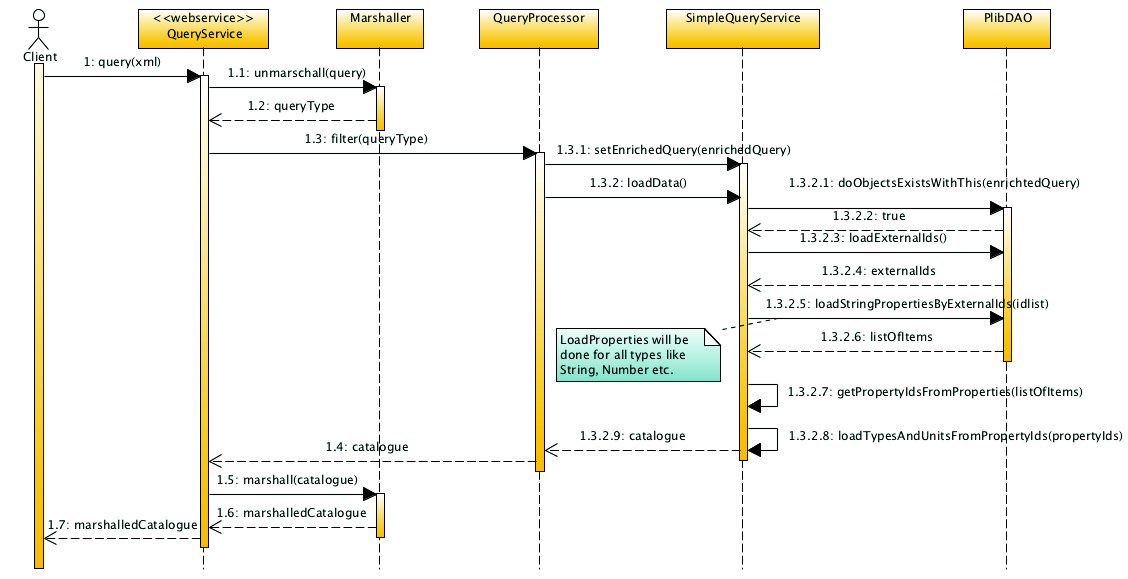
\includegraphics[width=0.99\textwidth]{images/plib_simple_query_sequence_diagram.jpg}
		\caption{Sequenzdiagramm Simple Query}
	\label{fig:sequenzdiagrammsimplequery}
\end{figure}

Der Ablauf einer Abfrage in der Applikation zeigt das Sequenzdiagramm in \autoref{fig:sequenzdiagrammsimplequery}. Hier werden beispielhaft anhand eines Simple Queries dargestellt, welche Klassen involviert sind. Die Aufrufe Richtung Datenbank von der Klasse PlibDAO werden der Einfachheit halber nicht dargestellt. 

\begin{table}[!hbt]\vspace{1ex}\centering\begin{tabular}{p{3cm}p{10cm}}
\hline
Schritt & Beschreibung\\
\hline
\hline
1 &  Der Klient sendet das Query-XML-File über den Webservice an den QueryService \\
\hline
1.1 &  Der Query wird umgewandelt in ein Java Modell \\
\hline
1.2 &  Das queryType Modell wird zurückgeliefert \\
\hline
1.3 &  Die Filter-Methode des QueryProcessors wird aufgerufen, nach Erkennung ob es sich um einen Simple Query oder Parametric Query handelt, wird der Query wird mit zusätzlichen Informationen angereichert. \\
\hline
1.3.1 &  Der angereicherte Query wird an den ausgewählten QueryService weitergeleitet.  \\
\hline
1.3.2 &  loadData wird aufgerufen um die Daten des Queries zu laden. \\
\hline
1.3.2.1 &  Es wird geprüft ob die angegebenen Objekte des Queries in der Datenbank verfügbar sind. \\
\hline
1.3.2 2 &  true wird zurückgeliefert. \\
\hline
1.3.2.3 &  Die external IDs der mittels IRDI übergebenen Objekte werden geladen. Hinweis: wie bereits erwähnt, liefern die Prozeduren keine Möglichkeit eine IRDI unmittelbar zu übergeben, sondern nur den external Identifier des konkreten Objektes. \\
\hline
1.3.2.4 &  Die externen IDs der Teile werden zurückgeliefert \\
\hline
1.3.2.5 &  Alle Eigenschaften der Teile werden geladen.  \\
\hline
1.3.2.6 &  Die Teile mit den Eigenschaften werden zurückgeliefert. \\
\hline
1.3.2.7 &  Alle IRDIs der Eigenschaften müssen aus den Ergebnissen ausgelesen und in das Katalog-Modell übertragen werden. \\
\hline
1.3.2.8 &  Alle Typen und Einheiten müssen aus den Ergebnissen ausgelesen und in das Katalog-Modell übertragen werden. \\
1.3.2.9 &  Das gefüllte Katalog-Modell wird zurückgeliefert. \\
\hline
1.4 &  Das gefüllte Katalog-Modell wird zurückgeliefert. \\
\hline
1.5 &  Das gefüllte Katalog-Modell wird in XML-Repräsentation umgewandelt. \\
\hline
1.6 &  Die XML-Repräsentation des Katalog-Modells wird zurückgeliefert. \\
\hline
1.7 &  Die XML-Repräsentation des Katalog-Modells wird an den Klient zurückgeliefert. \\
\hline
\end{tabular}
\caption{\label{tab.abfrageablauf}Erläuterung des Abfrageablaufes der Applikation}
\vspace{2ex}\end{table}
 

\subsection{Problemstellung - Daten der Teile Eigenschaften}\label{sec:problemdateneigenschaften}

Die genannten Prozeduren liefern die Daten der Eigenschaften eines spezifizierten Teiles nach IRDI. Die Liste der zurückgegebenen Daten scheint auf den ersten Blick ausreichend, denn man erhält die folgenden Eigenschaften der Prozedur

GET\_PROP\_VALS\_STRING:

\begin{itemize}
  \item IRDI
  \item VALUE
  \item UNIT
  \item PREFIX
  \item TOLERANCE
  \item VALUE\_ID
\end{itemize}

\enquote{VALUE} ist der Wert der Eigenschaft, \enquote{UNIT} die Einheit. Ein genauer Blick auf auf das Schema des Standards (siehe \autoref{lst:value_xsd} aus \autoref{kap:anhang_schema}), zeigt auf, dass es konkrete Typen für die Einheit des Wertes gibt, z.B. boolean\_value, complex\_value, composite\_value, controlled\_value usw., für eine komplette Liste siehe \autoref{lst:value_xsd}. 
Die Daten aus dem Response der Prozedur bezüglich UNIT, PREFIX und TOLERANCE kommen aus der Relation DO\_ADDITIONAL\_DATA, die mit der jeweiligen Datenbanktabelle der Eigenschaftswerte, das sind beispielsweise DO\_STRING, DO\_NUMBER, DO\_REFERENCES usw., verknüpft wird. Das bedeutet, dass einer Eigenschaft einer Instanz eines Teiles beispielsweise die Einheit (UNIT), gesetzt werden kann. Dies erscheint an dieser Stelle fragwürdig, da es bedeuten würde, für jede Instanz jeweils eine Einheit zu speichern. 
Es stellt sich hier das Problem, dass anhand des String-Wertes aus UNIT nicht klar ist, auf welchen Typen aus value.xsd gemappt werden soll. Es liegt ein Heterogenitätskonflikt der beiden Datenschemata vor.  
Ferner wurde festgestellt, dass über die Metadaten, nämlich der Relation DE\_PROPERTY über DE\_DATA\_TYPE auf DE\_UNIT und DE\_PREFIX verwiesen wird, womit allen Instanzen dieser Eigenschaft die Einheit (UNIT) und der Prefix (PREFIX) gesetzt werden kann. Dies erscheint sinnvoller und würde auch ein Mapping ermöglichen. 

\subsubsection{Lösung}

In einem Gespräch mit Karsten Mende\footnote{Karsten Mende ist der Studenten, welcher für die Datenbank- und Prozedurimplementierung verantwortlich ist. Zum Zeitpunkt des Verfassens dieser Arbeit, war die Abschlussarbeit von Herrn Mende noch nicht abgeschlossen.} wurde diese Situation besprochen. Herr Mende erläuterte, dass der Standard ISO 13584-42 \citep[vgl.][]{iso13584-42} die Möglichkeit gibt die Einheit der konkreten Instanzen von Eigenschaften zu überschreiben. Dies wurde von Herrn Mende implementiert. Auf Grund der Heterogenität und Repräsentation in Strings empfiehlt Herr Mende an dieser Stelle auf die Metadatenbeschreibungen von UNIT, PREFIX und TOLERANCE der Relationen DE\_PROPERTY, DE\_DATA\_TYPE, DE\_UNIT und DE\_PREFIX zurückzugreifen. 
Da dies sinnvoll erscheint und ferner die Implementierung vereinfacht, wurde dies in der Form umgesetzt. Es bleibt an dieser Stelle zu bemerken, dass für eine spätere Implementierung und Unterstützung dieser Funktionalität zu analyiseren ist, wie die Heterogenität zu lösen ist. Ggfs. muss dazu eine Mappingtabelle erstellt werden.

Fazit:
Zur Zeit werden folglich gesetzte Werte von UNIT, PREFIX und TOLERANCE in DO\_ADDTIONAL\_DATA ignoriert und nur die Metadatenrepräsentationen benutzt.  

\subsection{Problemstellung - Aufruf der Prozeduren mit Java}
Um die Prozeduren von Oracle aufzurufen wurde Spring Data Oracle eingesetzt. \index{Spring Data Oracle}

Die eigentlichen Hilfsprozeduren, welche von Karsten Mende zur Verfügung gestellt werden lieferten keine Rückgabewerte. Das \autoref{lst:spring_data_hilf} zeigt die erste Testimplementierung. 

Der Grund, weshalb keine Rückgabewerte geliefert werden ist, dass die Hilfsprozeduren Ausgaben mit der Oracle Funktion \enquote{dbms\_output.put\_line} erzeugen. Auf diese manuell erzeugten Ausgabetexte kann nicht zugegriffen werden. 

\begin{lstlisting}[caption=Spring Data Oracle - Klasse zum Aufruf der Hilfsprozeduren, language=, label=lst:spring_data_hilf]
package de.feu.plib.dao.procedures;

import org.apache.log4j.Logger;
import org.springframework.jdbc.core.SqlOutParameter;
import org.springframework.jdbc.core.SqlParameter;
import org.springframework.jdbc.object.StoredProcedure;

import javax.sql.DataSource;
import java.sql.Types;
import java.util.HashMap;
import java.util.Map;

/**
 * This class calls the HILF_GET_PROP_VALS procedure.
 * However, during tests I found out that we have no real out-parameter.
 * Thus either must be changed or Queries from the procedures must be used as simple sql.
 */
public class PropertyValuesStoredProcedure extends StoredProcedure {
    private static final String PROCEDURE_NAME = "PACK_PROPERTY.HILF_GET_PROP_VALS_STRING";

    /**
     * Logger instance
     */
    private static Logger LOGGER = Logger.getLogger(TestProcedure.class);

    public PropertyValuesStoredProcedure(DataSource ds) {
        super(ds, PROCEDURE_NAME);
        declareParameter(new SqlParameter("OBJ_ID", Types.VARCHAR));
        compile();
    }

    public String execute(String objectId) {
        Map in = new HashMap();
        in.put("OBJ_ID", objectId);
        Map out = execute(in);
        LOGGER.info("Output: " + out);
        if (!out.isEmpty())
            return out.get("OBJ_ID").toString();
        else
            return null;
    }
}

\end{lstlisting}

Im \autoref{lst:spring_data_hilf} leitet die Klasse PropertyValuesStoredProcedure von der Spring-Klasse StoredProcedure ab. Im Konstruktor werden die Parameter definiert, in diesem Falle lediglich OBJ\_ID als Externer Identifier. Ferner wird die Methode execute überschrieben, welche den Aufruf der Prozedur kapselt. 

\autoref{lst:spring_data_hilf_test} zeigt eine Testklasse, welche die Prozedur aufruft. Die Testklasse verfügt über zwei Testmethoden, testShowsThatWeHaveThatinDB und testShouldThrowExceptionAsExtIDIsNotInDB. 

\begin{description}
\item[ testShowsThatWeHaveThatinDB] Diese Methode übergibt einen gültigen und in der Datenbank vorhandenen Externen Identifier. Wird die Hilfsmethode über SQL direkt auf der Datenbank mit diesem Parameter aufgerufen, so wird folgendes ausgegeben:

  LIST\_STRING\_PROPS 1. Stelle
  Property-IRDI :  val : Euro
  
  LIST\_STRING\_PROPS 2. Stelle
  Property-IRDI :  val : 2008-12-31
  
  LIST\_STRING\_PROPS 3. Stelle
  Property-IRDI :  val : 170202
  
  LIST\_STRING\_PROPS 4. Stelle
  Property-IRDI :  val : 24-31-01-01
  
  LIST\_STRING\_PROPS 5. Stelle
  Property-IRDI :  val : Rundolf-75
  
  LIST\_STRING\_PROPS 6. Stelle
  Property-IRDI :  val : 2008-05-01
  
Es ist eine Liste mit sechs Eigenschaftswerten.
Wird die Prozedur über den Test aufgerufen, so ist der Testablauf zwar erfolgreich, allerdings liefert dieser kein Ergebnis zurück. Dieses Verhalten wurde nicht erwartet. 
  
\item[ testShouldThrowExceptionAsExtIDIsNotInDB] Diese Testmethode nutzt einen nicht vorhandenen Externen Identifier. Via SQL direkt auf der Datenbank ausgeführt liefert die Testmethode: \enquote{No Data found} zurück. 
Wird die Prozedur über den Test aufgerufen, so wird eine Exception geworfen, welche ebenfalls den Text  \enquote{No Data found} beinhaltet. Dies ist somit ein korrektes Verhalten. 
\end{description}

Der Grund, weshalb der Aufruf der Prozedur mit einem gültigen externen \gls{IRDI} keinen Wert zurückliefert ist der, dass die Hilfsmethoden mit dem Prefix 

HILF\_* (z.B. HILF\_GET\_PROP\_VAL\_STRING) 

in der Prozedurdefinition Ausgaben mittels 

DBMS\_OUTPUT.PUT\_LINE 

erzeugen. Das ist eine Oracle spezifische Funktion um Ausgaben zu erzeugen. Hierauf kann nicht zugegriffen werden. Ferner sind die Daten nicht strukturiert.   

\begin{lstlisting}[caption=Spring Data Oracle - Testklasse zum Aufruf der Hilfsprozeduren, language=java, label=lst:spring_data_hilf_test]
package de.feu.plib.dao.procedures;

import org.junit.After;
import org.junit.Before;
import org.junit.Test;
import org.junit.runner.RunWith;
import org.springframework.beans.factory.annotation.Autowired;
import org.springframework.test.context.ContextConfiguration;
import org.springframework.test.context.junit4.SpringJUnit4ClassRunner;

import javax.sql.DataSource;

@RunWith(SpringJUnit4ClassRunner.class)
@ContextConfiguration(locations = {"/beans.xml"})
public class PropertyValuesStoredProcedureIT {
    @Autowired
    javax.sql.DataSource ds;


    @Before
    public void setUp() throws Exception {
    }

    @After
    public void tearDown() throws Exception {
    }

    @Test
    public void testShowsThatWeHaveThatinDB() {

        PropertyValuesStoredProcedure propertyValuesStoredProcedure = new PropertyValuesStoredProcedure(ds);
        propertyValuesStoredProcedure.execute("EXT_50766884");

    }

    @Test(expected = RuntimeException.class)
    public void testShouldThrowExceptionAsExtIDIsNotInDB() {

        PropertyValuesStoredProcedure propertyValuesStoredProcedure = new PropertyValuesStoredProcedure(ds);
        propertyValuesStoredProcedure.execute("EXT_555");

    }

    public DataSource getDs() {
        return ds;
    }

    public void setDs(DataSource ds) {
        this.ds = ds;
    }

}

\end{lstlisting}

\subsubsection{Lösung}

Der nächste Test muss demnach eine Ebene tiefer ansetzen, und zwar dort, wo die Daten in Typstrukturen genutzt werden. Das sind die konkreten Prozeduren wie z.B. GET\_PROP\_VALS\_STRING. Diese liefern Tabellen vom Typ konkreter Rückgabetypen wie in \autoref{sec:abfrage_plib_prozeduren} beschrieben. 

Das \autoref{lst:spring_data_oracle} zeigt beispielhaft die Zugriffsklasse für die Prozedur 

GET\_PROP\_VALS\_STRING.

\begin{lstlisting}[caption=Spring Data Oracle - Aufruf der Prozeduren mit Rückgabetabellen, language=java, label=lst:spring_data_oracle]
package de.feu.plib.dao.procedures;

import java.util.HashMap;
import java.util.Map;

import javax.sql.DataSource;

import de.feu.plib.dao.procedures.types.PropStringNtt;
import oracle.jdbc.OracleTypes;
import org.apache.log4j.Logger;
import org.springframework.data.jdbc.support.oracle.SqlReturnSqlData;
import org.springframework.jdbc.core.SqlOutParameter;
import org.springframework.jdbc.core.SqlParameter;
import org.springframework.jdbc.object.StoredProcedure;

public class TestProcedure extends StoredProcedure {

    private static final String SQL = "PACK_PROPERTY.GET_PROP_VALS_STRING";

    /**
     * Logger instance
     */
    private static Logger LOGGER = Logger.getLogger(TestProcedure.class);

	public TestProcedure(DataSource ds) {
		super(ds, SQL);
		declareParameter(new SqlParameter("EXT_PROD_ID", OracleTypes.VARCHAR));

		declareParameter(new SqlOutParameter("OUTTABLE_STRING", OracleTypes.STRUCT, "PACK_PROPERTY.PROP_STRING_NTT", new SqlReturnSqlData(PropStringNtt.class)));
		compile();
	}

	public String execute(Long propertyId, Long is_cvp) {
		Map in = new HashMap();
		in.put("EXT_PROD_ID", propertyId);
        in.put("is_cvp", is_cvp);
		Map out = execute(in);
		if (!out.isEmpty())
			return out.get("message").toString();
		else
			return null;
	}

    public String execute(String propertyId) {
		Map in = new HashMap();
		in.put("EXT_PROD_ID", propertyId);
		Map out = execute(in);
		if (!out.isEmpty())
			return out.get("OUTTABLE_STRING").toString();
		else
			return null;
	}
}
\end{lstlisting}

\subsection{Problemstellung - RECORD-Types als Argumente werden nicht von Java JDBC unterstützt}

Im \autoref{lst:spring_data_oracle} wird ein Test dargestellt, der vermeintlich die Prozedur 

\enquote{GET\_PROP\_VALS\_STRING} 

aufrufen kann. Dies ist der nächste logische Schritt, welcher allerdings nicht funktioniert. Beim Aufruf der Prozedur von Java, wird eine Fehlermeldung zurückgegeben, welche den Rückgabetyp PACK\_PROPERTY.PROP\_STRING\_NTT nicht erkennt. 

Zur Erklärung dazu, PACK\_PROPERTY ist das von Herrn Mende definierte Paket, welches zum Ziel hat zusammengehörigen Prozeduren, Typen und Funktionen zu gruppieren. Die Erstellung von Paketen erhöht die Wart- und Lesbarkeit des Oracle-PL/SQL Codes. 

Eine Recherche hat ergeben, dass eine Oracle Prozedur welche RECORD-Types als IN oder OUT-Parameter benutzt, mittels Java JDBC-Treiber nicht aufgerufen werden können. 

Der SQLJ Developer's Guide and Reference sagt dazu \citep[Kap. 5][]{oracle-dev-guide}:

\begin{quotation}
\enquote{Oracle SQLJ and JDBC do not support calling arguments or return values of the PL/SQL BOOLEAN type or RECORD types. Also, when using the Thin driver, they do not support calling arguments or return values of PL/SQL TABLE types (known as indexed-by tables). TABLE types are supported for the OCI driver, however.}
\end{quotation}

\subsubsection{Lösung}

Es gibt mehrere Lösungsansätze. Der erste Ansatz ist autark zu lösen, ohne Anpassung der Prozeduren. Hierzu werden nicht die Prozeduren eingesetzt, sondern die benutzten SQL-Anfragen aus den Prozeduren werden eigenständig benutzt. 
Der Vorteil dieser Lösung ist, dass die Prozeduren nicht angepasst werden müssen. Der Nachteil ist allerdings, dass die Prozeduren, welche in der Arbeit von Herrn Mende entwickelt wurden in der Form gar nicht mehr genutzt werden. Das ist nicht das eigentliche Ziel, führt allerdings zum Ergebnis. 

Die erste Lösung wurde zu Testzwecken implementiert, siehe \autoref{lst:select_string}.

\begin{lstlisting}[caption=SELECT-Abfrage für String-Properties aus den Prozeduren, language=sql, label=lst:select_string]
SELECT 
    P.ID, 
    P.IRDI, 
    LOJ.VALUE, 
    LOJ.UNIT, 
    LOJ.PREFIX, 
    LOJ.TOLERANCE, 
    LOJ.VALUE_ID 
FROM 
    (SELECT 
    	DI_ID, 
	P_ID, 
	VALUE, 
	UNIT, 
	PREFIX, 
	TOLERANCE, 
	VALUE_ID
     FROM 
     	DO_STRING 
		LEFT OUTER JOIN 
			(SELECT 
				DI_ID, 
				P_ID, 
				UNIT, 
				PREFIX, 
				TOLERANCE, 
				VALUE_ID
			 FROM 
			 	DO_ADDITIONAL_DATA 
			 WHERE 
			 	ERR_CODE = 1)
			 USING (DI_ID, P_ID)
                          	WHERE (DI_ID =?) 
                          		AND (DO_STRING.ERR_CODE = 1))
                          	LOJ JOIN DE_PROPERTY P  
                          	ON LOJ.P_ID = P.ID
\end{lstlisting}

Wenngleich die Abfrage zum Ergebnis führt, so ist sie sehr komplex. Daher sollte wie geplant die Abfragekomplexität in der Prozedur gekapselt sein. Damit sind wir gleich beim zweiten Lösungsansatz. Hierbei müssen die Prozeduren angepasst und als Rückgabetyp einen OBJECT-Typ benutzt werden. 

Erst wurde die erste Lösung implementiert, um eine Basis für die weitere Entwicklung zu haben, denn für die zweite Lösung muss Herr Mende die Prozeduren anpassen. So konnte die Entwicklung fortgeführt werden und gleichzeitig Herr Mende die Änderungen für die zweite, gleichsam die empfohlene Lösung entwickeln. \autoref{lst:prop_string_typen} zeigt den von Herrn Mende neuen Beispieltypen PROP\_STRING\_OBJ. Analog zu den anderen Typen aus \autoref{sec:abfrage_plib_prozeduren} gibt es folglich weitere Typdefintionen wie z.B. PROP\_NUMBER\_OBJ oder PROP\_REFERENZ\_OBJ. 
Die Prozeduren mit den RECORD Typen wurden beibehalten und neue Prozeduren entwickelt. Die Benamung ist GET\_OBJ\_STRING, GET\_OBJ\_NUMBER usw..

\begin{lstlisting}[caption=PROP\_STRING\_OBJ Typen, language=sql, label=lst:prop_string_typen]
create or replace
  TYPE        "PROP_STRING_OBJ_T" AS OBJECT(
  P_IRDI    VARCHAR2(4000),
  "VALUE"   VARCHAR2(4000),
  unit      VARCHAR2(30),
  prefix    VARCHAR2(30),
  tolerance NUMBER,
  VALUE_ID  NUMBER
);

create or replace
TYPE   "PROP_STRING_OBJ_NTT"  AS TABLE OF  "PROP_STRING_OBJ_T";
\end{lstlisting}

\subsection{Problemstellung - Fehlender Fremdschlüsselidentifier in Prozedurrückgabedaten}

Wie bereits in \autoref{sec:problemdateneigenschaften} beschrieben liefern die Prozeduren mit den folgenden Attributen zurück: 

IRDI, VALUE, UNIT, PREFIX, TOLERANCE, VALUE\_ID

Ferner wird aufgezeigt, dass die Tabellen DE\_PROPERTY über DE\_DATA\_TYPE auf DE\_UNIT und DE\_PREFIX an alle relevanten Daten für das semantische Mapping kommt. Es stellt sich aber das Problem, dass die Rückgabedaten keinen Identifier beinhalten (P\_ID - Property ID), über welche die Tabellen miteinander verknüpft werden können (Join). 
 
\subsubsection{Lösung}

Es gibt zwei Lösungsansätze. Die erste Lösung ist, weitere SQL Anfragen zu stellen um die benötigten Daten zu erfragen. Nachteilig ist an dieser Lösung, dass bereits für die Ermittlung des Externen Identifiers aus \autoref{sec:problemidentifier} zusätzliche Anfragen nötig sind. In diesem Fall kommen weitere hinzu. 

Die andere Lösung ist die Anpassung der Prozeduren und Rückgabetypen, so dass unmittelbar die Property ID mitgeliefert wird. Das hat den Vorteil, dass keine weitere SQL-Anfrage an die Datenbank gesendet werden muss. Innerhalb der Prozedur wird ein weiteres Attribut selektiert. 

Es wurde die zweite Lösung gewählt. Hierbei müssen alle Typdefinitionen angepasst werden, siehe beispielhaft \autoref{lst:prop_string_typen_mod}. Dazu wird die Property ID eingefügt:

\enquote{P\_ID	 NUMBER}.

 \begin{lstlisting}[caption=PROP\_STRING\_OBJ Typanpassung, language=sql, label=lst:prop_string_typen_mod]
create or replace
  TYPE        "PROP_STRING_OBJ_T" AS OBJECT(
  P_ID	NUMBER
  P_IRDI    VARCHAR2(4000),
  "VALUE"   VARCHAR2(4000),
  unit      VARCHAR2(30),
  prefix    VARCHAR2(30),
  tolerance NUMBER,
  VALUE_ID  NUMBER
);

create or replace
TYPE   "PROP_STRING_OBJ_NTT"  AS TABLE OF  "PROP_STRING_OBJ_T";
\end{lstlisting}

Das \autoref{lst:get_obj_string_anpassung} zeigt die gesamte GET\_OBJ\_STRING Prozedur samt Anpassung. 

 \begin{lstlisting}[caption=GET\_OBJ\_STRING Anpassung auf Property ID, language=sql, label=lst:get_obj_string_anpassung]

PROCEDURE GET_OBJ_STRING (
       EXT_PROD_ID                 IN VARCHAR2,
       OUTTBL_OBJ_STRING           OUT PROP_STRING_OBJ_NTT,
       CREATED_VIEW                IN NUMBER := NULL
       )
IS
       
       CURSOR CUR_DO_STRING (IN_OBJ_ID NUMBER) 
       IS
       SELECT p.id, P.IRDI, LOJ.VALUE, LOJ.UNIT, LOJ.PREFIX, LOJ.TOLERANCE, LOJ.VALUE_ID 
       FROM (SELECT DI_ID, P_ID,  VALUE, UNIT, PREFIX, TOLERANCE, VALUE_ID 
             FROM DO_STRING LEFT OUTER JOIN (SELECT DI_ID, P_ID, UNIT, PREFIX, TOLERANCE, VALUE_ID
                                             FROM DO_ADDITIONAL_DATA 
                                             WHERE ERR_CODE = 1)
             USING (DI_ID, P_ID) 
             WHERE (DI_ID =IN_OBJ_ID) AND (DO_STRING.ERR_CODE = 1))LOJ JOIN DE_PROPERTY P
             ON LOJ.P_ID = P.ID
       ORDER BY P.IRDI;      
 
  OBJ_ID_NR               NUMBER;
  OUTTABLE_STRING         PROP_STRING_NTT := PROP_STRING_NTT();
  OUTTBL_OBJ_STRING_ELEM  PROP_STRING_OBJ_T := PROP_STRING_OBJ_T(NULL, NULL, NULL, NULL, NULL, NULL, NULL);
  I                       INTEGER;
  EMPTY_OUTTBL_OBJ_STRING PROP_STRING_OBJ_NTT := PROP_STRING_OBJ_NTT();

BEGIN
  OUTTBL_OBJ_STRING :=  EMPTY_OUTTBL_OBJ_STRING;
   
  IF CREATED_VIEW IS NULL THEN
    EXECUTE IMMEDIATE 'SELECT DI_ID FROM DO_OBJECT WHERE EXT_PROD_ID = ''' || EXT_PROD_ID || ''' AND CREATED_VIEW IS NULL' INTO OBJ_ID_NR;
  ELSE
    EXECUTE IMMEDIATE 'SELECT DI_ID FROM DO_OBJECT WHERE EXT_PROD_ID = ''' || EXT_PROD_ID || ''' AND CREATED_VIEW = ' || CREATED_VIEW INTO OBJ_ID_NR ;
  END IF;
      
  OPEN CUR_DO_STRING(OBJ_ID_NR);
  FETCH CUR_DO_STRING BULK COLLECT INTO OUTTABLE_STRING; 
  CLOSE CUR_DO_STRING; 
  
  IF OUTTABLE_STRING.FIRST IS NULL THEN
    DBMS_OUTPUT.PUT_LINE('OUTTABLE_STRING ist leer!');
  ELSE 
    DBMS_OUTPUT.PUT_LINE('OUTTABLE_STRING ist NICHT leer!');
    FOR I IN OUTTABLE_STRING.FIRST .. OUTTABLE_STRING.LAST LOOP
      
      DBMS_OUTPUT.PUT_LINE('OUTTABLE_STRING(I).PROP_IRDI: '||  OUTTABLE_STRING(I).PROP_IRDI);
      OUTTBL_OBJ_STRING_ELEM.P_ID := OUTTABLE_STRING(I).PROP_ID;
      OUTTBL_OBJ_STRING_ELEM.P_IRDI := OUTTABLE_STRING(I).PROP_IRDI;
      OUTTBL_OBJ_STRING_ELEM.VALUE := OUTTABLE_STRING(I).VAL;
      OUTTBL_OBJ_STRING_ELEM.UNIT := OUTTABLE_STRING(I).UNIT;
      OUTTBL_OBJ_STRING_ELEM.PREFIX := OUTTABLE_STRING(I).PREFIX;
      OUTTBL_OBJ_STRING_ELEM.TOLERANCE := OUTTABLE_STRING(I).TOLERANCE;
      OUTTBL_OBJ_STRING_ELEM.VALUE_ID := OUTTABLE_STRING(I).VALUE_ID;
      OUTTBL_OBJ_STRING.EXTEND;
      OUTTBL_OBJ_STRING(OUTTBL_OBJ_STRING.LAST) := OUTTBL_OBJ_STRING_ELEM;
      DBMS_OUTPUT.PUT_LINE('Wertzuweisung an OUTTBL_OBJ_STRING erfolgreich!');
    END LOOP; 
  END IF;
   
END GET_OBJ_STRING;
\end{lstlisting}
 
Es müssen drei Stellen angepasst werden: 

\begin{itemize}
\item Das SELECT Statement für die Rückgabe, so dass die Property ID übergeben wird: 
  \begin{description}
  \item[vorher] SELECT \\
  P.IRDI, \\
  LOJ.VALUE, \\ 
  LOJ.UNIT, \\
  LOJ.PREFIX, \\ 
  LOJ.TOLERANCE, \\
  LOJ.VALUE\_ID \\
  ...
  \item[nachher] SELECT \\
  P.ID, \\
  P.IRDI, \\ 
  LOJ.VALUE, \\ 
  LOJ.UNIT, \\
  LOJ.PREFIX, \\ 
  LOJ.TOLERANCE, \\ 
  LOJ.VALUE\_ID \\
  ...
  \end{description}
\item Die Erweiterung bei Instanzierung des Tabelleneintrages für den Tabellentypen um ein Attribut (NULL hinzugefügt): 
  \begin{description}
  \item[vorher] OUTTBL\_OBJ\_STRING\_ELEM  PROP\_STRING\_OBJ\_T :=  \\
  PROP\_STRING\_OBJ\_T(NULL, NULL, NULL, NULL, NULL, NULL);
  \item[nachher] OUTTBL\_OBJ\_STRING\_ELEM  PROP\_STRING\_OBJ\_T :=  \\
  PROP\_STRING\_OBJ\_T(NULL, NULL, NULL, NULL, NULL, NULL, NULL);
  \end{description}
\item Hinzufügen des Mappings von der RECORD-Tabelle auf den OBJECT-Typen:
  \begin{description}
  \item[vorher] -
  \item[nachher] OUTTBL\_OBJ\_STRING\_ELEM.P\_ID := OUTTABLE\_STRING(I).PROP\_ID;  
  \end{description}
\end{itemize}
 
\section{Fehlerbehandlung}

Treten während der Verarbeitung Fehler auf, wie z.B. ein Validierungsfehler des übergebenen XML Queries, so ergibt sich das Problem, dass diese Fehlermeldung nicht an den Klienten zurückgegeben werden kann. Das ist nicht möglich, da das aktuelle Schema der Rückgabedatei \enquote{query.xsd}  (siehe \autoref{sec:query_xsd}) kein Modell für Fehlernachrichten beinhaltet. 
Dieses Verhalten ist genau genommen korrekt, denn hier wird ein Datenmodell beschrieben und Kontext- und Zusatzinformationen gehören streng genommen nicht in dieses Modell, sondern sollten über eine darüber liegende Ebene verarbeitet werden.

Dies ist in der Lösung mit \gls{REST}ful \gls{Webservice} nicht sinnvoll möglich, daher bieten sich zwei Möglichkeiten an. Die erste Möglichkeit wäre beim Auftreten eines Fehlers in der Verarbeitung immer einen leeren Katalog zurückzuliefern. Der Vorteil der Lösung ist die Einfachheit. Der Nachteil ist, dass nach wie vor keinerlei Fehlerinformation an den Klienten zurückgeliefert wird. 

Die zweite Möglichkeit ist ein weiteres Schema zu erstellen, dieses im Katalog-Schema zu referenzieren. In diesem \enquote{Fehler-Schema} wird dann ein Fehlertyp definiert, welcher Fehlernachrichten aufnehmen kann. Der Vorteil dieser Lösung ist, dass es einfach umzusetzen und in das vorhandenen Katalog-Schema zu integrieren ist. Der Nachteil ist, dass es eine Anpassung der Katalog-Schemas bedeutet. 

Um Anhand der Antwort (Katalogdaten) einen Fehler überhaupt erkennen zu können, wurde die zweite Lösung gewählt. Die \autoref{lst:error_schema} zeigt die Schemadatei error.xsd, welche einen Typen definiert (errorType) der zwei Fehlertexte beinhalten kann, shortErrorMessageType und longErrorMessageType. 

 \begin{lstlisting}[caption=Fehlerbehandlung - Error Schemadatei, language=xml, label=lst:error_schema]
<?xml version="1.0" encoding="UTF-8"?>
<!--
error.xsd - Additional simple Schema for adding to another Schema. Allows Error Messages. 
-->
<xs:schema xmlns:xs="http://www.w3.org/2001/XMLSchema" xmlns:err="error" targetNamespace="error" elementFormDefault="qualified" attributeFormDefault="unqualified">
	<xs:complexType name="errorType">
		<xs:sequence>
			<xs:element name="shortErrorMessage" type="err:shortErrorMessageType" />
			<xs:element name="longErrorMessage" type="err:longErrorMessageType" />
		</xs:sequence>
	</xs:complexType>
	<xs:simpleType name="shortErrorMessageType">
		<xs:restriction base="xs:string"/>
	</xs:simpleType>
	<xs:simpleType name="longErrorMessageType">
		<xs:restriction base="xs:string"/>
	</xs:simpleType>
</xs:schema>
\end{lstlisting}

Diese lässt sich in die Katalog-Schemadatei einbinden mittels

\lstinline[basicstyle=\ttfamily\small\mdseries]{<xs:import namespace="error" schemaLocation="error.xsd" /> }

Anschließend wird ein globales Error-Element angegeben:

\lstinline[basicstyle=\ttfamily\small\mdseries]{<xs:element name="error" type="err:errorType" />}

Schließlich wird der Catalogue-Type neben dem Item-Type noch durch den Error Type erweitert, das zeigt \autoref{lst:error_catalogue_erweitern}.

 \begin{lstlisting}[caption=Fehlerbehandlung - Catalogue Type erweitern, language=xml, label=lst:error_catalogue_erweitern]
	<xs:complexType name="catalogue_Type">
		<xs:sequence>
			<xs:element ref="cat:item" minOccurs="0" maxOccurs="unbounded"/>
			<xs:element ref="cat:error" minOccurs="0" maxOccurs="1"/>
		</xs:sequence>
	</xs:complexType> 
	
\end{lstlisting} 

Das \autoref{lst:error_catalogue_beispiel} zeigt eine Beispielantwort einer Fehlermeldung. Hier wurde ein ungültige IRDI im Query gesendet. Die shortErrorMessage besagt, dass es sich um einen Fehler beim Unmarshalling handelt. Der gesamte Java-Stacktrace aus der aufgetretenen Exception im Programm wird in der longErrorMessage angegeben. Hier kann genau nach der Ursache des Fehlers geforscht werden. In diesem Fall findet man folgende Fehlernachricht:

\enquote{Caused by: org.xml.sax.SAXParseException: cvc-pattern-valid: Value '01x73x-1#01-AAA352#4' is not facet-valid with respect to pattern ... for type 'IRDI_type'.}

Es ist ein Fehler bei der Validierung der IRDI aufgetreten. Diese entspricht nicht dem erlaubten Muster.

 \begin{lstlisting}[caption=Fehlerbehandlung - Beispielantwort mit Validierungsfehler=xml, label=lst:error_catalogue_beispiel]
?xml version="1.0" encoding="UTF-8" standalone="yes"?>
<catalogue xmlns:ns2="urn:iso:std:iso:ts:29002:-4:ed-1:tech:xml-schema:basic" xmlns="urn:iso:std:iso:ts:29002:-10:ed-1:tech:xml-schema:catalogue" xmlns:ns4="error" xmlns:ns3="urn:iso:std:iso:ts:29002:-10:ed-1:tech:xml-schema:value">
    <error>
        <ns4:shortErrorMessage>Error occured during unmarshalling of xml</ns4:shortErrorMessage>
        <ns4:longErrorMessage>java.lang.RuntimeException: Error during unmarshalling of XML.
	at de.feu.plib.xml.XMLMarshallerImpl.unmarshallXML(XMLMarshallerImpl.java:63)
	at de.feu.plib.webservice.rest.QueryRESTService.unmarshall(QueryRESTService.java:151)
	at de.feu.plib.webservice.rest.QueryRESTService.query(QueryRESTService.java:91)
	at sun.reflect.NativeMethodAccessorImpl.invoke0(Native Method)
	at sun.reflect.NativeMethodAccessorImpl.invoke(NativeMethodAccessorImpl.java:39)
	at sun.reflect.DelegatingMethodAccessorImpl.invoke(DelegatingMethodAccessorImpl.java:25)
	at java.lang.reflect.Method.invoke(Method.java:597)
	at com.sun.jersey.spi.container.JavaMethodInvokerFactory$1.invoke(JavaMethodInvokerFactory.java:60)
	at com.sun.jersey.server.impl.model.method.dispatch.AbstractResourceMethodDispatchProvider$TypeOutInvoker._dispatch(AbstractResourceMethodDispatchProvider.java:185)
	at com.sun.jersey.server.impl.model.method.dispatch.ResourceJavaMethodDispatcher.dispatch(ResourceJavaMethodDispatcher.java:75)
	at com.sun.jersey.server.impl.uri.rules.HttpMethodRule.accept(HttpMethodRule.java:288)
	at com.sun.jersey.server.impl.uri.rules.RightHandPathRule.accept(RightHandPathRule.java:147)
	at com.sun.jersey.server.impl.uri.rules.ResourceClassRule.accept(ResourceClassRule.java:108)
	at com.sun.jersey.server.impl.uri.rules.RightHandPathRule.accept(RightHandPathRule.java:147)
	at com.sun.jersey.server.impl.uri.rules.RootResourceClassesRule.accept(RootResourceClassesRule.java:84)
	at com.sun.jersey.server.impl.application.WebApplicationImpl._handleRequest(WebApplicationImpl.java:1469)
	at com.sun.jersey.server.impl.application.WebApplicationImpl._handleRequest(WebApplicationImpl.java:1400)
	at com.sun.jersey.server.impl.application.WebApplicationImpl.handleRequest(WebApplicationImpl.java:1349)
	at com.sun.jersey.server.impl.application.WebApplicationImpl.handleRequest(WebApplicationImpl.java:1339)
	at com.sun.jersey.spi.container.servlet.WebComponent.service(WebComponent.java:416)
	at com.sun.jersey.spi.container.servlet.ServletContainer.service(ServletContainer.java:537)
	at com.sun.jersey.spi.container.servlet.ServletContainer.service(ServletContainer.java:699)
	at javax.servlet.http.HttpServlet.service(HttpServlet.java:728)
	at org.apache.catalina.core.ApplicationFilterChain.internalDoFilter(ApplicationFilterChain.java:305)
	at org.apache.catalina.core.ApplicationFilterChain.doFilter(ApplicationFilterChain.java:210)
	at org.apache.catalina.core.StandardWrapperValve.invoke(StandardWrapperValve.java:222)
	at org.apache.catalina.core.StandardContextValve.invoke(StandardContextValve.java:123)
	at org.apache.catalina.authenticator.AuthenticatorBase.invoke(AuthenticatorBase.java:502)
	at org.apache.catalina.core.StandardHostValve.invoke(StandardHostValve.java:171)
	at org.apache.catalina.valves.ErrorReportValve.invoke(ErrorReportValve.java:99)
	at org.apache.catalina.valves.AccessLogValve.invoke(AccessLogValve.java:953)
	at org.apache.catalina.core.StandardEngineValve.invoke(StandardEngineValve.java:118)
	at org.apache.catalina.connector.CoyoteAdapter.service(CoyoteAdapter.java:408)
	at org.apache.coyote.http11.AbstractHttp11Processor.process(AbstractHttp11Processor.java:1023)
	at org.apache.coyote.AbstractProtocol$AbstractConnectionHandler.process(AbstractProtocol.java:589)
	at org.apache.tomcat.util.net.JIoEndpoint$SocketProcessor.run(JIoEndpoint.java:310)
	at java.util.concurrent.ThreadPoolExecutor$Worker.runTask(ThreadPoolExecutor.java:895)
	at java.util.concurrent.ThreadPoolExecutor$Worker.run(ThreadPoolExecutor.java:918)
	at java.lang.Thread.run(Thread.java:695)
Caused by: org.xml.sax.SAXParseException: cvc-pattern-valid: Value '01x73x-1#01-AAA352#4' is not facet-valid with respect to pattern '[0-9]{4}-[0-9A-Z:_\.]{1,35}(-[0-9A-Z:_\.]{1,35}(-[0-9A-Z]{1,1}(-[0-9A-Z:_\.]{1,70})?)?)?(#[0-9A-Z]{2,2}-[0-9A-Z:_\.]{1,131}#[0-9]{1,10})?|[0-9]{4}-[0-9A-Z:_\.]{1,35}(-[0-9A-Z:_\.]{1,35})?--[0-9A-Z:_\.]{1,70}(#[0-9A-Z]{2,2}-[0-9A-Z:_\.]{1,131}#[0-9]{1,10})?|[0-9]{4}-[0-9A-Z:_\.]{1,35}---[0-9A-Z:_\.]{1,70}(#[0-9A-Z]{2,2}-[0-9A-Z:_\.]{1,131}#[0-9]{1,10})?' for type 'IRDI_type'.
	at com.sun.org.apache.xerces.internal.util.ErrorHandlerWrapper.createSAXParseException(ErrorHandlerWrapper.java:195)
	at com.sun.org.apache.xerces.internal.util.ErrorHandlerWrapper.error(ErrorHandlerWrapper.java:131)
	at com.sun.org.apache.xerces.internal.impl.XMLErrorReporter.reportError(XMLErrorReporter.java:384)
	at com.sun.org.apache.xerces.internal.impl.XMLErrorReporter.reportError(XMLErrorReporter.java:318)
	at com.sun.org.apache.xerces.internal.impl.xs.XMLSchemaValidator$XSIErrorReporter.reportError(XMLSchemaValidator.java:423)
	at com.sun.org.apache.xerces.internal.impl.xs.XMLSchemaValidator.reportSchemaError(XMLSchemaValidator.java:3188)
	at com.sun.org.apache.xerces.internal.impl.xs.XMLSchemaValidator.elementLocallyValidType(XMLSchemaValidator.java:3103)
	at com.sun.org.apache.xerces.internal.impl.xs.XMLSchemaValidator.processElementContent(XMLSchemaValidator.java:3013)
	at com.sun.org.apache.xerces.internal.impl.xs.XMLSchemaValidator.handleEndElement(XMLSchemaValidator.java:2156)
	at com.sun.org.apache.xerces.internal.impl.xs.XMLSchemaValidator.endElement(XMLSchemaValidator.java:824)
	at com.sun.org.apache.xerces.internal.jaxp.validation.ValidatorHandlerImpl.endElement(ValidatorHandlerImpl.java:566)
	at com.sun.xml.bind.v2.runtime.unmarshaller.ValidatingUnmarshaller.endElement(ValidatingUnmarshaller.java:106)
	at com.sun.xml.bind.v2.runtime.unmarshaller.SAXConnector.endElement(SAXConnector.java:158)
	at com.sun.org.apache.xerces.internal.parsers.AbstractSAXParser.endElement(AbstractSAXParser.java:604)
	at com.sun.org.apache.xerces.internal.impl.XMLDocumentFragmentScannerImpl.scanEndElement(XMLDocumentFragmentScannerImpl.java:1789)
	at com.sun.org.apache.xerces.internal.impl.XMLDocumentFragmentScannerImpl$FragmentContentDriver.next(XMLDocumentFragmentScannerImpl.java:2950)
	at com.sun.org.apache.xerces.internal.impl.XMLDocumentScannerImpl.next(XMLDocumentScannerImpl.java:647)
	at com.sun.org.apache.xerces.internal.impl.XMLNSDocumentScannerImpl.next(XMLNSDocumentScannerImpl.java:140)
	at com.sun.org.apache.xerces.internal.impl.XMLDocumentFragmentScannerImpl.scanDocument(XMLDocumentFragmentScannerImpl.java:513)
	at com.sun.org.apache.xerces.internal.parsers.XML11Configuration.parse(XML11Configuration.java:815)
	at com.sun.org.apache.xerces.internal.parsers.XML11Configuration.parse(XML11Configuration.java:744)
	at com.sun.org.apache.xerces.internal.parsers.XMLParser.parse(XMLParser.java:128)
	at com.sun.org.apache.xerces.internal.parsers.AbstractSAXParser.parse(AbstractSAXParser.java:1208)
	at com.sun.org.apache.xerces.internal.jaxp.SAXParserImpl$JAXPSAXParser.parse(SAXParserImpl.java:543)
	at com.sun.xml.bind.v2.runtime.unmarshaller.UnmarshallerImpl.unmarshal0(UnmarshallerImpl.java:218)
	at com.sun.xml.bind.v2.runtime.unmarshaller.UnmarshallerImpl.unmarshal(UnmarshallerImpl.java:196)
	at com.sun.xml.bind.v2.runtime.unmarshaller.UnmarshallerImpl.unmarshal(UnmarshallerImpl.java:250)
	at de.feu.plib.xml.XMLMarshallerImpl.unmarshallXML(XMLMarshallerImpl.java:57)
	... 38 more
</ns4:longErrorMessage>
    </error>
</catalogue>
\end{lstlisting} 

\section{SOAP Webservice}

Um beide Technologien miteinander zu vergleichen wurde nach der \gls{REST}ful \gls{Webservice}-Implementierung noch ein \gls{SOAP}-\gls{Webservice} implementiert. 

Das Ergebnis ist, dass basierend auf der vorhandenen Implementierung ein weiterer Webservice in einer anderen Technologie mit recht geringem Aufwand erstellt werden kann. Im Rahmen der \gls{REST}ful \gls{Webservice}-Implementierung wurden bereits alle vorbereitenden Maßnahmen, wie Modellgenerierung aus den Schemadateien, getroffen. 
 
Mehr Informationen zur Implementierung und Beispielquellcode des \gls{SOAP}-\glspl{Webservice} gibt das\autoref{kap:anhang_soap_webservice}. 
 
\section{Zusammenfassung des Kapitels}

Zunächst wird das Configuration Management erläutert, dazu gehört die Auswahl der Werkzeuge, Prozesse, Build-Umgebung, Frameworks und Plattformen. Es wird kurz auf das Thema Testen eingegangen und anhand einiger Beispiele erläutert. Da ein \gls{REST}ful \gls{Webservice} entwickelt wird, ist eine Beschreibung dieses Webservices Bestandteil des Kapitels. Es wird aufgezeigt wie ein  \gls{REST}ful \gls{Webservice} mit Hilfe des Frameworks Jersey entwickelt wird. 
Der nächste Schritt ist die Betrachtung des Datenmodells. Die Anfrage und die Antwort des  \glspl{Webservice} ist mittels Schema beschrieben. Die Herausforderung ist die Umwandlung der XML-Daten gemäß Schema in ein Modell der Programmiersprache zu Weiterverarbeitung.  
Der wichtigste Punkt ist die Abfrage der \gls{Oracle} \gls{PLIB}-Prozeduren. Hier ergeben sich diverse Problemstellungen wie semantische Heterogenität, fehlende Daten bei Eingabe- und Ausgabeschnittstelle der Prozeduren als auch technische Schwierigkeiten, wie die fehlende Unterstützung von RECORD-Typen bei Abfrage mit Java JDBC.
Die aufgetretenen Probleme zeigen auf, dass bei der Implementierung und Integration von Schnittstellen mit Problemen zu rechnen ist. Die Prozeduren wurden nicht mit Augenmerk auf die ISO 29002-31 entwickelt und weisen dadurch eine deutliche Heterogenität zu den tatsächlich benötigen Daten auf. Die Ergebnisse der Implementierung zeigen ferner, dass Abstraktionen behilflich sind. Würden die Prozeduren gemäß den tatsächlich benötigen Daten und mit Betrachtung der ISO 29002-31 angepasst, ließen sich zusätzliche Datenbankabfragen vermeiden und die Komplexität in der Business Logik Schicht verringern. Dennoch vereinfachen die Prozeduren den Zugriff enorm, denn wie \autoref{lst:select_string} zeigt, kapseln die Prozeduren komplexe Anfragen und vereinfachen die Schnittstelle zur Datenbank. 
Das Fehlerhandling wird in den Modellen nicht betrachtet. Um Informationen beim Auftreten von Fehlern an den Klienten zu senden, wurde eine Fehler-Schemadatei mit Fehlertypen erstellt und das Katalog-Schema angepasst, so dass als Antwort ggfs. Fehlertexte mitgesendet werden können. 
Auf die vorhandene Implementierung der Business Logik und der Modelle der Schemata lässt sich sehr einfach ein weiterer \gls{Webservice} basierend auf SOAP implementieren. Das bedeutet, dass die oberste Schicht ausgetauscht werden kann. Es wurden beide Technologien verwendet, welche die gleiche Business Logik aufrufen. 

